\documentclass[a4paper]{article}

\usepackage[english]{babel}
\usepackage{amsmath}
\usepackage{amssymb}
\usepackage{dsfont}
\usepackage{graphicx}
\usepackage{listings}
\usepackage[hyphens]{url}
\usepackage{titling}
\usepackage{varwidth}
\usepackage{hyperref}
\usepackage{color} %red, green, blue, yellow, cyan, magenta, black, white
\definecolor{mygreen}{RGB}{28,172,0} % color values Red, Green, Blue
\definecolor{mylilas}{RGB}{170,55,241}



\usepackage{geometry}
 \geometry{
 a4paper,
 total={165mm,257mm},
 left=20mm,
 top=20mm,
 }

\title{Natural Computing\\Assignment 1}
\author{
  Christoph Schmidl\\ s4226887\\      \texttt{c.schmidl@student.ru.nl}
  \and
  Koen Vijverberg\\ s1337\\     \texttt{koen@example.com}
  \and
  Alex\\	s1337\\	\texttt{alex@example.com}
}
\date{\today}

\begin{document}
\maketitle


\subsection*{Exercises on Evolutionary Computation}

\begin{enumerate}

	% Task 1	
	\item A generational GA has a population size of 100 individuals; uses fitness proportional
selection without elitisms; and after $t$ generation has a mean population fitness of 76.
There is one copy of the current best member, which has fitness 157.

	\begin{enumerate}
		\item What is the expectation for the number of copies of the best individual in the mating pool?\\
		\textbf{Solution:}\\
		
		\item What is the probability that there will be no copis of the best individual in the mating pool?\\
		\textbf{Solution:}\\
		
	
	\end{enumerate}

	% Task 2	
	\item Given the fitness function $f(x) = x^2$, calculate the probability of selecting the individuals $x = 3, x = 5$ and $x = 7$, using roulette wheel selection. Calculate the probability of selecting the same individuals when the fitness function is $f1(x) = f(x) + 8$. Which fitness function yields a lower selection pressure?\\
	\textbf{Solution:}\\	



	% Task 3
	\item The Counting Ones problem amounts to find a bit string whose sum of its entries is maximum. This easy problem is used to illustrate the difference between Monte-Carlo search and a simple genetic algorithm.\\
	Monte-Carlo search for binary problems works as follows.
	
	\begin{enumerate}
		\item Start with a random bit sequence.
		\item If it is equal to the goal sequence then stop, otherwise repeat the process from step (a).
	\end{enumerate}
	
	Implement a Monte-Carlo search algorithm for the Counting Ones problem. Let the input take the following arguments:
	
	\begin{itemize}
		\item the objective function
		\item the length $n$ of the bitstrings
		\item the maximum number of fitness function evaluations
\end{itemize}

Let the algorithm produce as outputs:

\begin{itemize}
	\item the best individual found by the algorithm
	\item the fitness of the best individual
\end{itemize}

\begin{enumerate}
	\item Use $n = 100$ and for a run of 1500 iterations, plot the best fitness against the elapsed number of iterations.\\
	\textbf{Solution:}\\
	
	\item Now do ten runs. How many times the algorithm finds the optimum? Almost never.\\
	\textbf{Solution:}\\
	
	
\end{enumerate}			
	
	% Task 4
	\item A simple (1 + 1)-GA for binary problems works as follows.
	
		\begin{enumerate}
			\item Randomly generate a bit sequence $x$
			\item Create a copy of $x$ and invert each of its bits with probability $p$. Let $x_m$ be the result.
			\item If $x_m$ is closer to the goal sequence than $x$ then replace $x$ with $x_m$
			\item Repeat the process from step (b) with the new $x$ until the goal sequence is reached.
		\end{enumerate}

	Implement a simple (1 + 1)-GA for solving the Counting Ones problem, using the same approach as with the Monte-Carlo search algorithm.
	
	\begin{enumerate}
		\item Use $n = 100$ and a mutation rate $p = 1/n$. For a run of 1500 iterations, plot the best fitness against the elapsed number of iterations.\\
		\textbf{Solution:}\\
		
		\item Now do ten runs. How many times the algorithm finds the optimum?\\
		\textbf{Solution:}\\
		
		
		\item Is there a difference in performance compared to the Monte-Carlo Search algorithm? Justify your answer.\\
		\textbf{Solution:}\\
	\end{enumerate}
	
	
	% Task 5
	\item (Genetic Programming) Give a suitable function, terminal set and s-expression for the following logical formula:
	
	\begin{equation}
		(x \wedge true) \rightarrow ((x \vee y) \vee (z \leftrightarrow (x \wedge y))) \notag
	\end{equation}
	\textbf{Solution:}\\

	Function set: $\{\vee,\wedge,\rightarrow,\leftrightarrow\}$\\
	Terminal set: $\{x,y,z,true,(false)\}$
	\begin{figure}[ht!]
	\centering
  	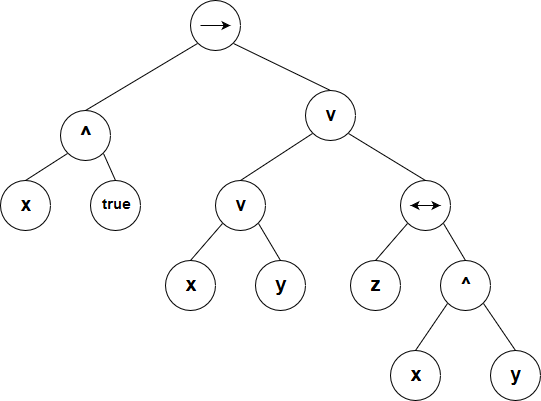
\includegraphics[width=0.6\textwidth]{images/s-expression.png}
	\end{figure}

	% Task 6
	\item (Genetic Programming) Implement a GP program for finding a symbolic expression that fits the following data:

	\begin{figure}[ht!]
	\centering
  	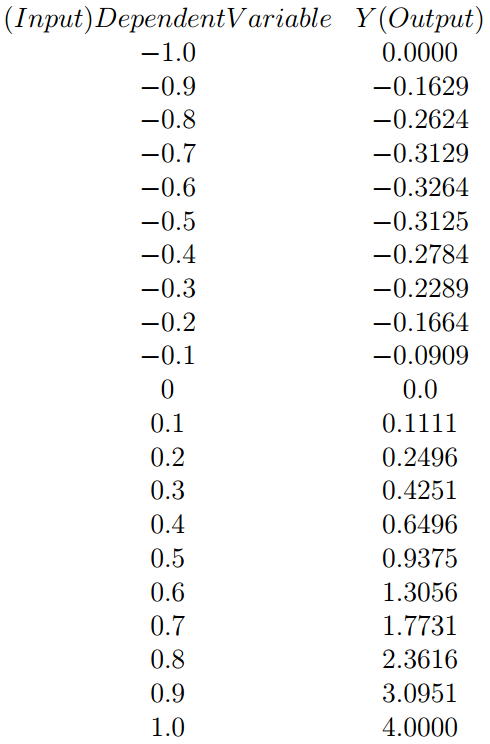
\includegraphics[width=0.35\textwidth]{images/table.PNG}
	\end{figure}	

with the following paramter setting:
\begin{itemize}
	\item population size: 1000
	\item function set: $\{+,-,*,log,exp,sin,cos,div \}$
	\item terminal set: $x$
	\item initialization: full
	\item number of generations: 50
	\item crossover probability: 0.7
	\item mutation probability: 0
	\item fitness: - sum of absolute errors
\end{itemize}

You can use an existing GP framework: see for instance list of implementation frameworks mentioned in the syllabus.\\

Plot the following:

\begin{enumerate}
	\item best of generatation fitness (y-axis) versus generation (x-axis)\\
	\textbf{Solution:}\\
	\begin{figure}[ht!]
	\centering
  	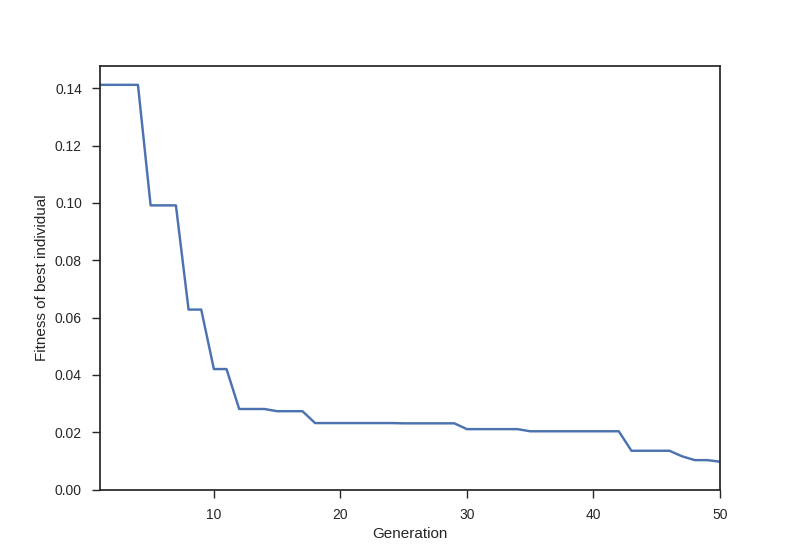
\includegraphics[width=0.5\textwidth]{SR_fit.png}
	\end{figure}
	
	\item best of generation size (y-axis) versus generation (x-axis).\\
	\textbf{Solution:}\\
	\begin{figure}[ht!]
	\centering
  	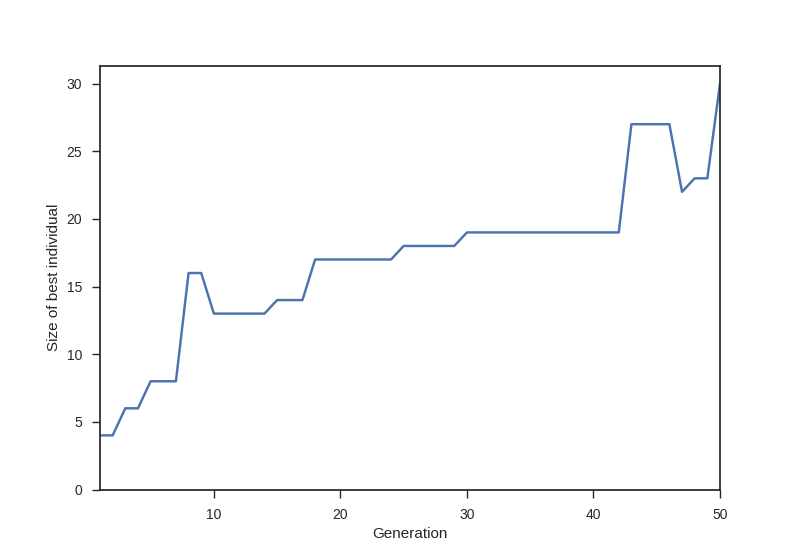
\includegraphics[width=0.5\textwidth]{SR_sz.png}
	\end{figure}
	
\end{enumerate}

Can you observe any undesirable phenomenon from these plots? In case of positive answer, explain how you would try to overcome the corresponding problem (you can refer to the literature).\\
\textbf{Solution:}\\
The size keeps increasing. It seems that the algorithm is overfitting a 'wrong' solution by adding extra terms such that it fits the data. A possible countermeasure is to incorporate the size of the tree into the fitness and punish large trees.

The code regarding this exercise can be found at our Git Repository:

\begin{itemize}
	\item Pure Python file: \url{https://github.com/ChristophSchmidl/natural-computing/blob/master/assignment-1/Symb_reg.py}
\end{itemize}	
		

\end{enumerate}




\end{document}
